\section{DP capabilities under visual perturbations}\label{sec:results}
We first evaluate in Section~\ref{sec:vis_impact} the performance of the LeRobot DP under the visual perturbations presented in Section~\ref{sec:experiments}.
Then, in Section~\ref{sec:solve_pb}, we present and evaluate different strategies aimed at addressing the model's lack of robustness to occlusions.

\subsection{Impact of visual perturbations on DP capabilities}\label{sec:vis_impact}
To evaluate the capabilities of LeRobot's DP under different visual perturbations, we conducted experiments on $20$ random seeds of the PushT environment.
The success rate is measured across varying action horizons under the input conditions described in Section~\ref{sec:experiments}.
The results are summarized in Table~\ref{tab:success_rates}.

\paragraph{Effect of Action Horizon}

Table~\ref{tab:success_rates} results indicate that increasing the action horizon generally enhances the policy's success rate under clear input conditions.
Specifically, the success rate improves from 20\% at an action horizon of 1 to 70\% at a horizon of 16.
This trend suggests that the diffusion policy benefits from longer prediction horizons, possibly due to better planning and anticipation of future states.
Furthemore, we find similar results as the ones promised by LeRobot in Table~\ref{tab:evaluation_results}.
However, it is important to keep in mind that in practice, within potentially dynamic environments,
a horizon that is too large results in a loss of reactivity for the agent.
A trade-off must be found to ensure the best performance based on the frequency of changes in the environment.

\paragraph{Robustness to Gaussian Noise}
Under Gaussian noise conditions, the policy maintains a performance level comparable to, and in some cases slightly exceeding, that with clear inputs.
Notably, at an action horizon of 8, the success rate peaks at 70\%, matching the best performance under clear conditions.
This resilience indicates that the LeRobot diffusion policy training effectively handles sensor-level noise, likely owing to its data augmentation as presented in Section~\ref{sec:pretrained_model}.
The fact that the optimal sequence length is shorter aligns with our observation on reactivity: the
agent quickly replans its trajectories and performs well on average.

\paragraph{Sensitivity to Occlusions}
In contrast, the policy's performance drops to 0\% success across all action horizons when faced with black patch occlusions.
The random placement of the occluding patch may block critical visual information necessary for task completion.
This sharp decline highlights the policy's vulnerability to occlusions and suggests that it heavily relies on uncorrupted visual inputs to make accurate predictions.
Since the success rate is no longer a suitable metric for evaluating the agent's performance,
we relied on the mean maximum coverage. Although the coverage is very minimal, we observed that the best
results were achieved with a horizon of length 1: the agent performs better by averaging multiple
predictions rather than following a single uncertain generation.
Furthermore, we observe degraded performance even when the black patch does not affect the visual
information used, i.e., the agent, the object, and the target. This case illustrates poor handling
of situations outside the training distribution: the agent's movements are fuzzy, or even almost random.

\begin{table}[!htb]
    \centering
    \caption{Success rates for different action horizons (steps) under various input conditions.}
    \label{tab:success_rates}
    \begin{tabular}{c|c|c|c}
    \hline
    \textbf{Action Horizon} & \textbf{Clear} & \textbf{Gaussian} & \textbf{Patch} \\
    \hline
    1 & 0.2 & 0.2 & 0.0 \\
    2 & 0.3 & 0.45 & 0.0 \\
    5 & 0.35 & 0.4 & 0.0 \\
    8 & 0.65 & \textbf{0.7} & 0.0 \\
    16 & \textbf{0.7} & 0.5 & 0.0 \\
    \hline
    \end{tabular}
\end{table}

The experiments reveal that while the diffusion policy is robust to certain types of visual perturbations like Gaussian noise, it is significantly affected by occlusions, a case that is not present during training time.
The inability to handle occluded inputs indicates a limitation in the model's capacity to infer missing information or focus on unoccluded regions.
These findings underscore the need for strategies to enhance the policy's robustness to occlusions, such as incorporating data augmentation with occlusions during training, or leveraging additional sensory modalities.
%In the Annex~\TODO{ref annex}, we provide a deeped analysis of the results by looking at the reward during the rollout of the episodes.

In the following section, we explore potential methods to overcome the challenges posed by occlusions and improve the diffusion policy's performance in the presence of such visual disturbances.



\subsection{Overcoming the Patch Problem}\label{sec:solve_pb}

In this section, we present our strategies to mitigate the performance degradation caused by visual occlusions, focusing specifically on addressing the challenges posed by the black patch.

The performance drop observed in Table~\ref{tab:success_rates} when black patch occlusions are introduced highlights the vulnerability of the DP model to visual perturbations.
To tackle this issue, we propose two solutions.

The first solution involves augmenting the training dataset with examples containing occlusions, thereby improving the policy's robustness to such challenges.
By exposing the model to occlusions during training, it can learn to generalize better to scenarios with similar disruptions.

The other solutions explore working at test time only, using simple heuristics.
This allows us to study whether satisfactory occlusion robustness can still be achieved with simple approaches.

Instead of evaluating performance based on the success rate as seen in Table~\ref{tab:success_rates}, Table~\ref{tab:res_ov_patch}
focuses on the average max reward obtained during the rollout of the episodes.
The average max reward is almost equivalent to the average max coverage. The reward is defined as:
$$
\text{reward} = \text{clip}\left(\text{coverage} / \text{max coverage}, 0, 1\right)
$$
where $\text{clip}(x, a, b)$ is a function that clips $x$ to be between $a$ and $b$, and $\text{max coverage}$
is set to $0.95$.
This shift in evaluation metric is motivated by the high cost of training a diffusion policy from scratch for 200,000 steps, which is necessary to achieve a good success rate.
However, the average reward serves as a reliable performance indicator even with fewer training steps (as few as 5,000).
This makes it a practical alternative for studying the impact of our proposed strategies while minimizing training costs.

\paragraph{(a) Adding Random Erasing (RE) Data Augmentation}
The first approach introduces random erasing data augmentation~\cite{zhong2020random} into the training process.
This technique involves randomly erasing parts of the input image during training, effectively simulating occlusions and forcing the model to become more robust to such disruptions.
An example of this augmentation is illustrated in Figure~\ref{fig:erasing}.
The model was trained using this augmentation for 10,000 and 20,000 training steps, corresponding to approximately 2.45 and 4.9 hours of training time, respectively, on a Kaggle P100 GPU.
As shown in Table~\ref{tab:res_ov_patch} by the RE results, the model begins to recover good average rewards from 10,000 training steps.
This demonstrates the effectiveness of random erasing in improving the model's performance while maintaining a reasonable computational cost.

\begin{figure}[!htb]
  \centering
  \begin{tabular}{cc}
    
\includegraphics[width=0.49\linewidth]{figures/fig_erasing.pdf}
  \end{tabular}
  \caption{Image with random erasing data augmentation.}
  \label{fig:erasing}
\end{figure}


\paragraph{(b) Combining Gaussian Noise (GN) with Occlusions}
This approach, illustrated by Figure~\ref{fig:patch_noise}, involves degrading the overall image quality by adding Gaussian noise (mean $0$, standard deviation $0.1$) to it, alongside the black patch occlusion.
The motivation of this experiment is to desensitize the neural network to the black patch by reducing its relative impact on the input image.
As simple visual data augmentation are already applied at training time, the noisy image forces the model to rely less on specific visual details within the input.
As shown in Table~\ref{tab:res_ov_patch} by the GN average max reward, this strategy results in no improvement in the model's ability to recover rewards compared to using the black patch alone.
\begin{figure}[!htb]
    \centering
    \begin{tabular}{cc}
      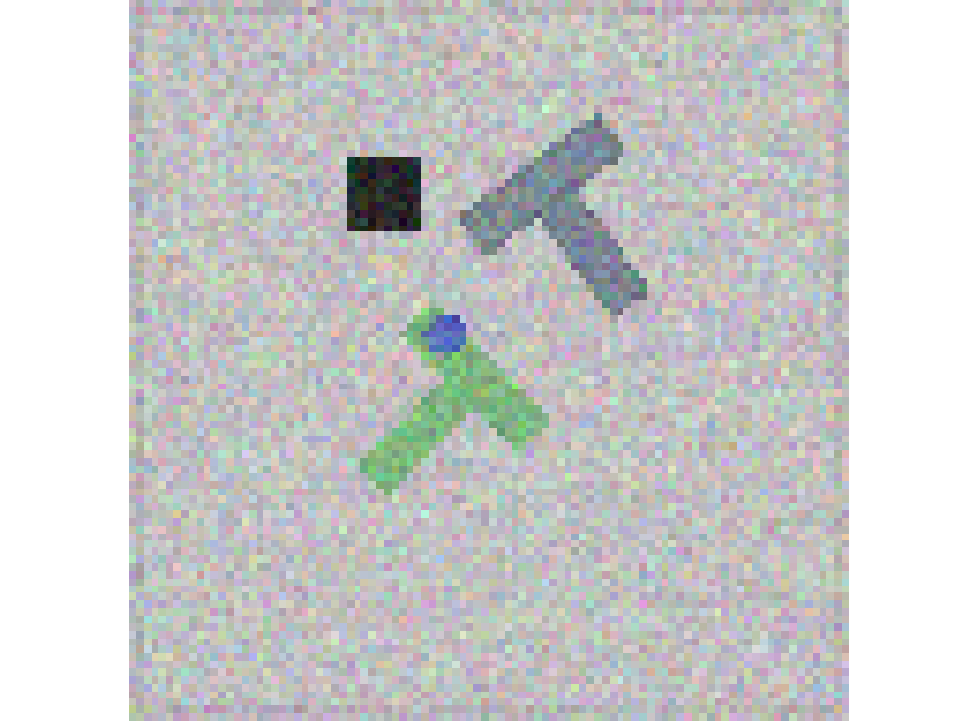
\includegraphics[width=0.49\linewidth]{figures/illustration_patch_noise.pdf}
    \end{tabular}
    \caption{Image with Gaussian noise and a 10x10 occlusion patch.}
    \label{fig:patch_noise}

\end{figure}

\paragraph{(c) Dynamic Adjustment (DA) of Action Sequence Length}
This last approach targets the model's action generation process.
By dynamically reducing the action sequence length during task execution, we hypothesize that the model becomes more responsive to changes in the visual input, allowing it to adapt better to challenging scenarios such as mooving black patches.
We evaluate this strategy using both linear and exponential decay schedules for action sequence length, as illustrated in Figure~\ref{fig:dynamic_adjustment}.
The results presented as DA in Table~\ref{tab:res_ov_patch} show that reducing the action sequence length doesn't improve the policy's performance over time.

\begin{figure}[!htb]
    \centering
    \begin{tabular}{cc}
      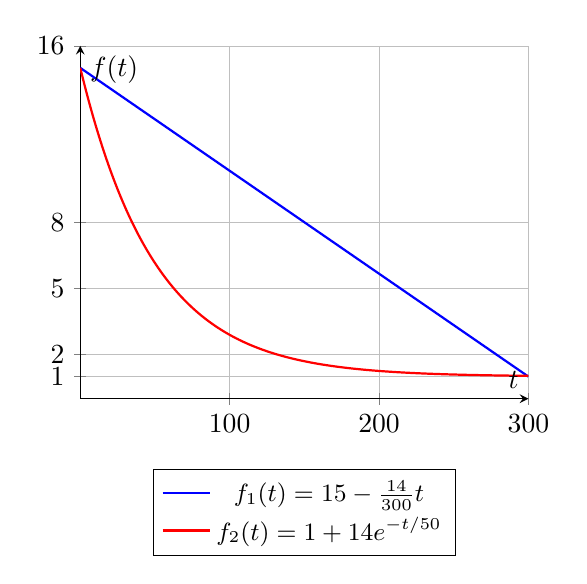
\begin{tikzpicture}
        \begin{axis}[
          width=0.6\linewidth,          % Span the full width of the column
          height=0.5\linewidth,         % Fixed height
          xlabel={$t$},                % Label for the x-axis
          ylabel={$f(t)$},             % Label for the y-axis
          xmin=-0.1, xmax=300,         % Range for x-axis
          ymin=0, ymax=16,             % Range for y-axis
          xtick={0,100,200,300},       % Define specific x-axis ticks      
          ytick={1,2, 5, 8, 16},       % Define specific y-axis ticks      
          grid=both,                   % Display grid lines
          grid style={line width=.1pt, draw=gray!10},
          major grid style={line width=.2pt,draw=gray!50},
          axis lines=middle,           % Position the axes in the middle
          legend style={font=\small, at={(0.5,-0.2)}, anchor=north}, % Position legend below plot
        ]
          % Plotting the Linear Function
          \addplot[
            domain=0:300, 
            samples=300, 
            color=blue, 
            thick
          ]{15 - (14 / 300)*x};
          \addlegendentry{$f_1(t) = 15 - \frac{14}{300} t$}
          
          % Plotting the Exponential Decay Function
          \addplot[
            domain=0:300,
            samples=300,
            color=red,
            thick
          ]{1 + 14 * exp(-x / 50)};
          \addlegendentry{$f_2(t) = 1 + 14 e^{-t/50}$}
        \end{axis}
      \end{tikzpicture}
      % 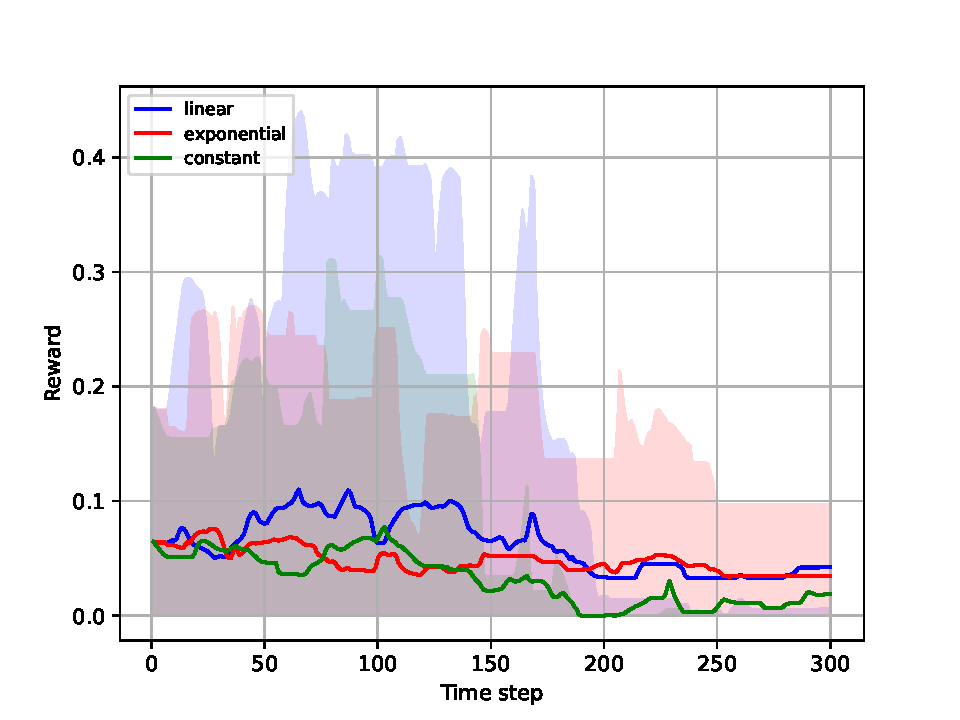
\includegraphics[width=0.49\linewidth]{figures/decrease_length.pdf} \\
    \end{tabular}
    \caption{Adjustement functions used for the dynamic adjustment of action sequence length across time steps.}
    \label{fig:dynamic_adjustment}
\end{figure}


\begin{table}[!htb]
  \centering
  \begin{tabular}{c|c}
  \hline
   & Avg max reward \\
  \hline
  LeRobot & 0.19 \\
  GN & 0.23 \\
  DA (linear) & 0.15  \\
  DA (exponential) & 0.27  \\
  RE (10k) & 0.52 \\
  RE (20k) & \textbf{0.59} \\
  \hline
  \end{tabular}
  \caption{Average max reward of the proposed stragies to overcome the black patch problem.
  "LeRobot" result is the average max reward of the Hugging Face LeRobot model.}
  \label{tab:res_ov_patch}
\end{table}

Table~\ref{tab:res_ov_patch} results demonstrate the effectiveness of data augmentation in significantly improving the model's robustness.
Indeed, we obtain average max reward values similar to those achieved when training the model for 5k steps
without augmentations and evaluating it on unperturbed images (around 0.6).
Additionally, the analysis reveals that even with fewer training steps, the model retains an acceptable performance level, offering a computationally efficient alternative.